\documentclass[11pt]{article}
\usepackage{classTools}
\usepackage{graphicx}

\draftfalse

\begin{document}

\psHeader{6}{Wed Oct. 26, 2022 (11:59pm)}

\textbf{Your name: Nikhil Datar}

\textbf{Collaborators: Adam Zhou}

\textbf{No. of late days used on previous psets: 5}

\textbf{No. of late days used after including this pset: }

\begin{enumerate}
 \item (Matching Algorithms) 

 One practical application of matching algorithms is planning logistics, like in the following example from (fictional) ridesharing service Lyber in (real) New York City's Times Square.  When a customer books a Lyber ride, the ride request is sent to a Lyber server and combined with others to create a schematic 

 like the one drawn in the map below:


\begin{figure}[H]
    \centering
    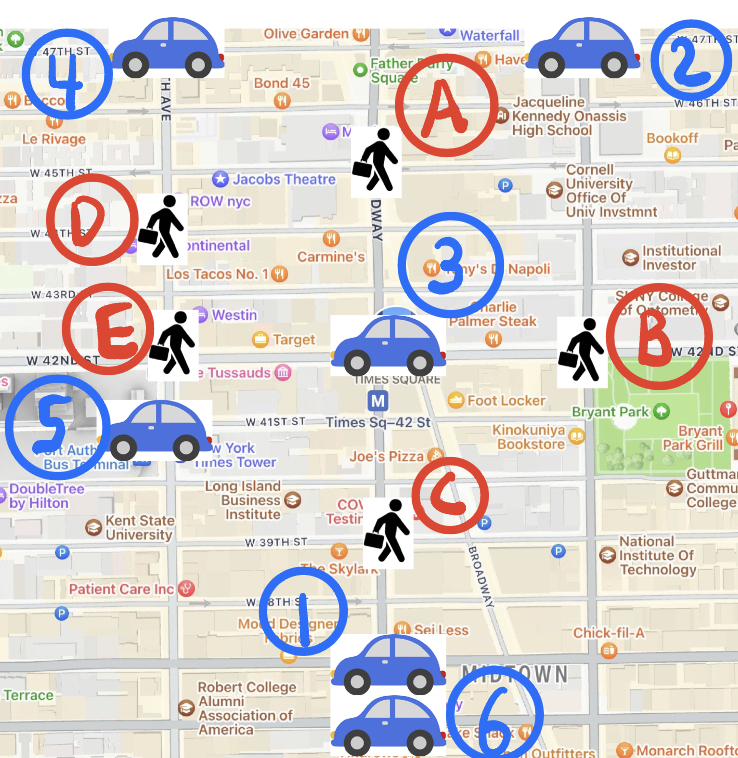
\includegraphics[width=0.87\textwidth]{NYC-map-zoomed-light.jpeg}
    \label{fig:travel_time_graph}
\end{figure}

Given a schematic like this, Lyber's goal is to serve as many customers (labeled A--E in the map) as possible, by assigning each one to a driver (labeled 1--6 in the map). For simplicity, each customer and driver is at an intersection, and assume driving between adjacent streets (vertical segment) takes 30 seconds, and driving between adjacent avenues (horizontal segments) takes 1 minute. However, the one twist is that they want to make sure that \textit{no customer is waiting for longer than 2 minutes}.  They also do not want to assign a driver to more than one customer at once, since serving a single customer can take more than 2 minutes.

    \begin{enumerate}
    \item To perform the assignment, they reduce to Maximum Matching in bipartite graphs.  Draw a bipartite graph corresponding to the drivers and customers in the map above. \\
    
    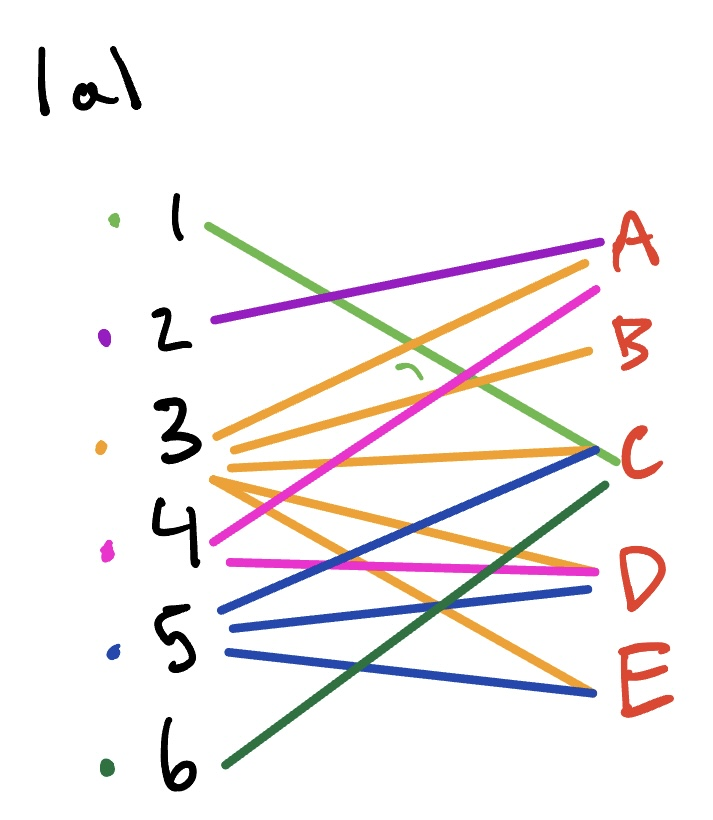
\includegraphics[width=.75\textwidth]{fall2022/psets/ps6/IMG_0009.jpg}

    
    \item The Lyber app first prioritizes customers on Broadway, so they initially assign customer $A$ to driver 3 and customer $C$ to driver 5. Using the algorithm from class, find a \textit{maximum matching} in the bipartite matching graph you've drawn, starting from the initial matching of $A$ to 3 and $C$ to 5. Draw pictures showing the sequence of matchings and augmenting paths you find. (No need to break down the steps of the algorithm to find the augmenting paths.) \\
    
    We use the maximum matching algorithm provided in class in order to solve for the maximum match given the initial state. \\
    
    Within this graph, we denote edges from the previous match iteration or initial match with red lines, and new edges formed from the augmented path with green lines. We circle edges from the previous iteraion (red lines) that are contained in the augmenting path with yellow to keep track of which edges will be removed to form the next match iteration. With that said, the steps/augmented paths followed are described below. \\
    
    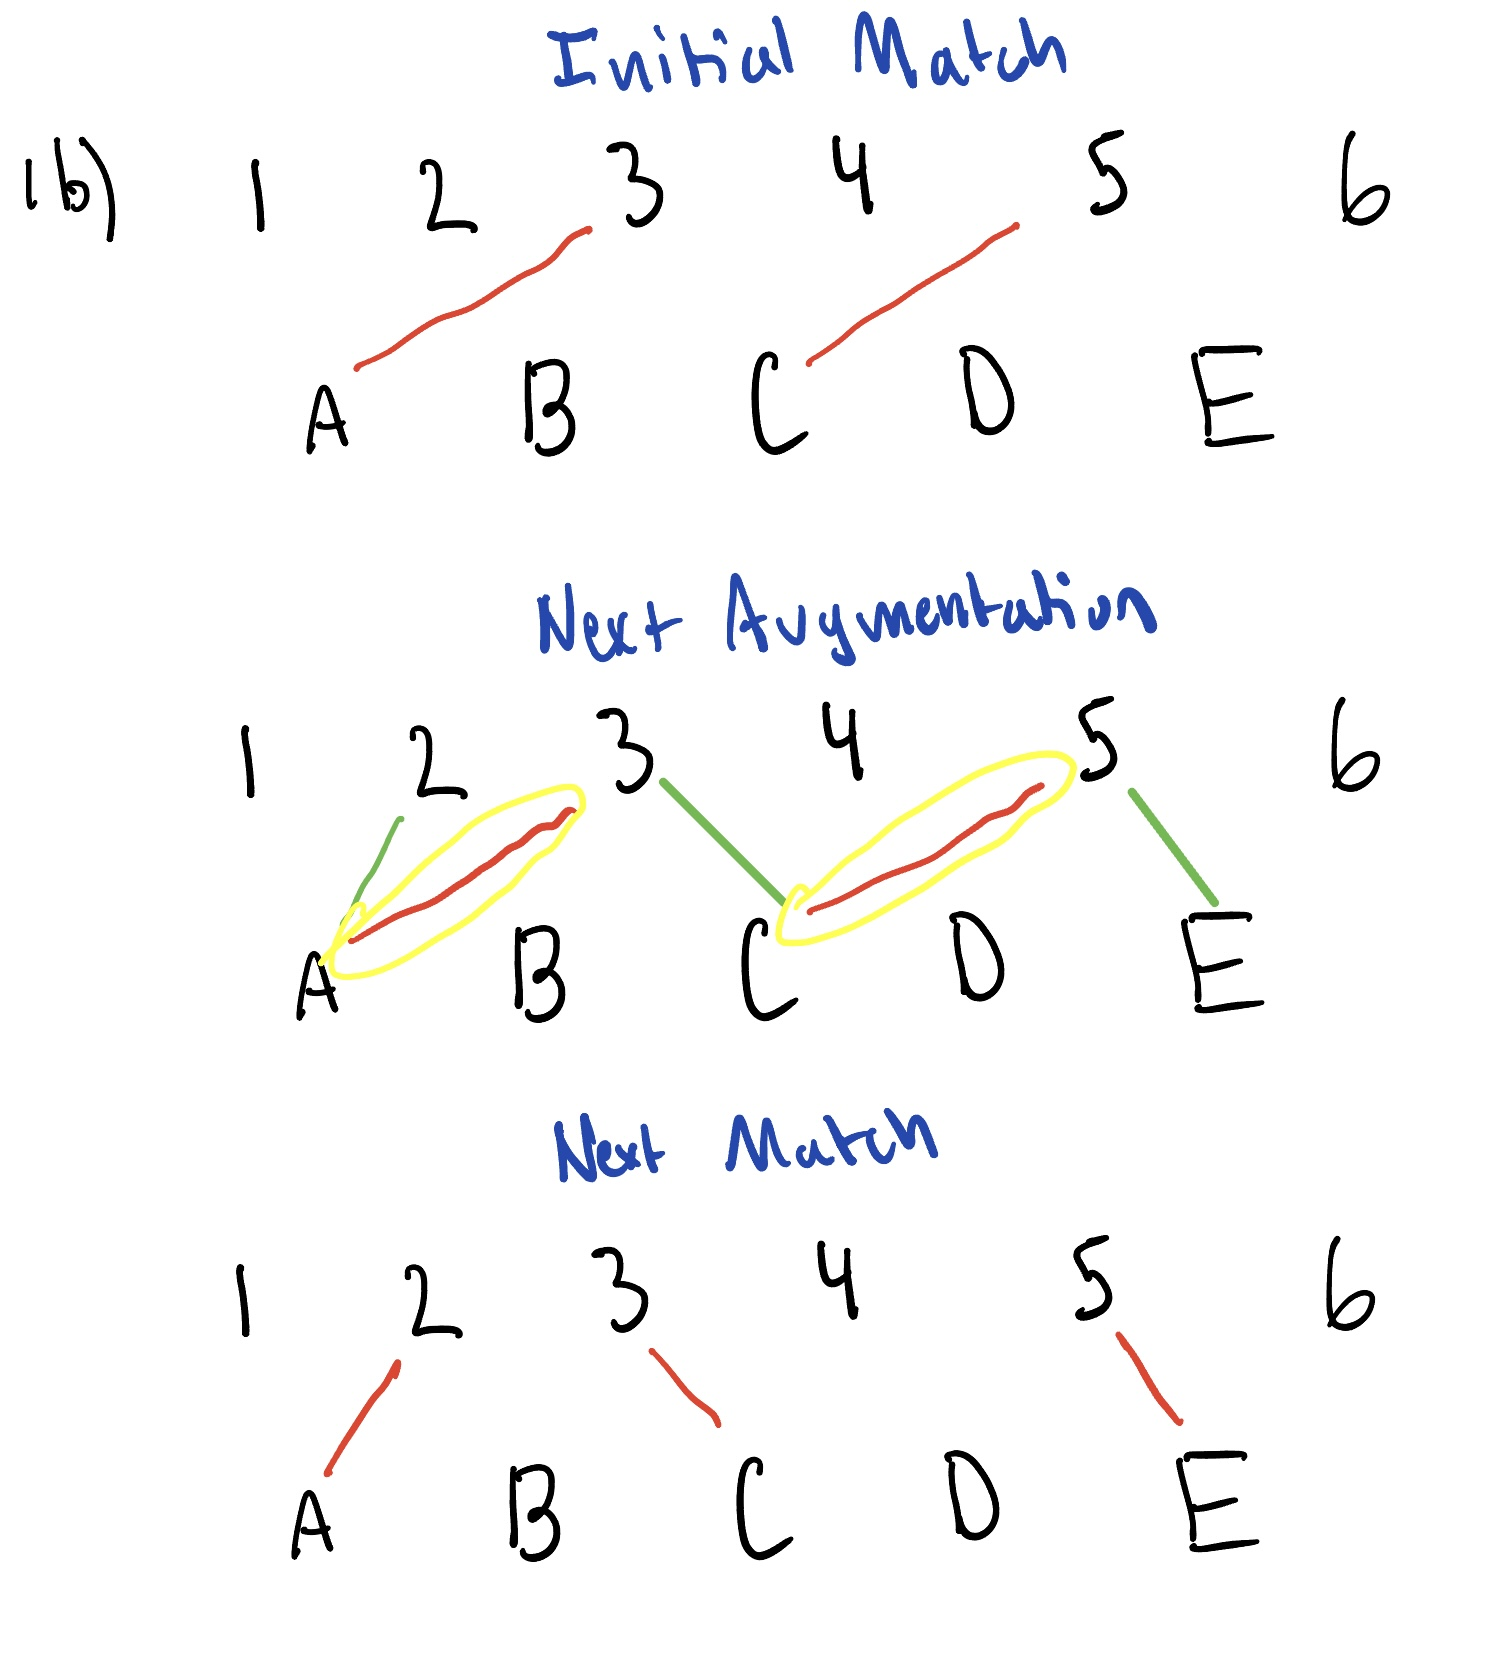
\includegraphics[width=.75\textwidth]{fall2022/psets/ps6/IMG_0010.jpg}\\
    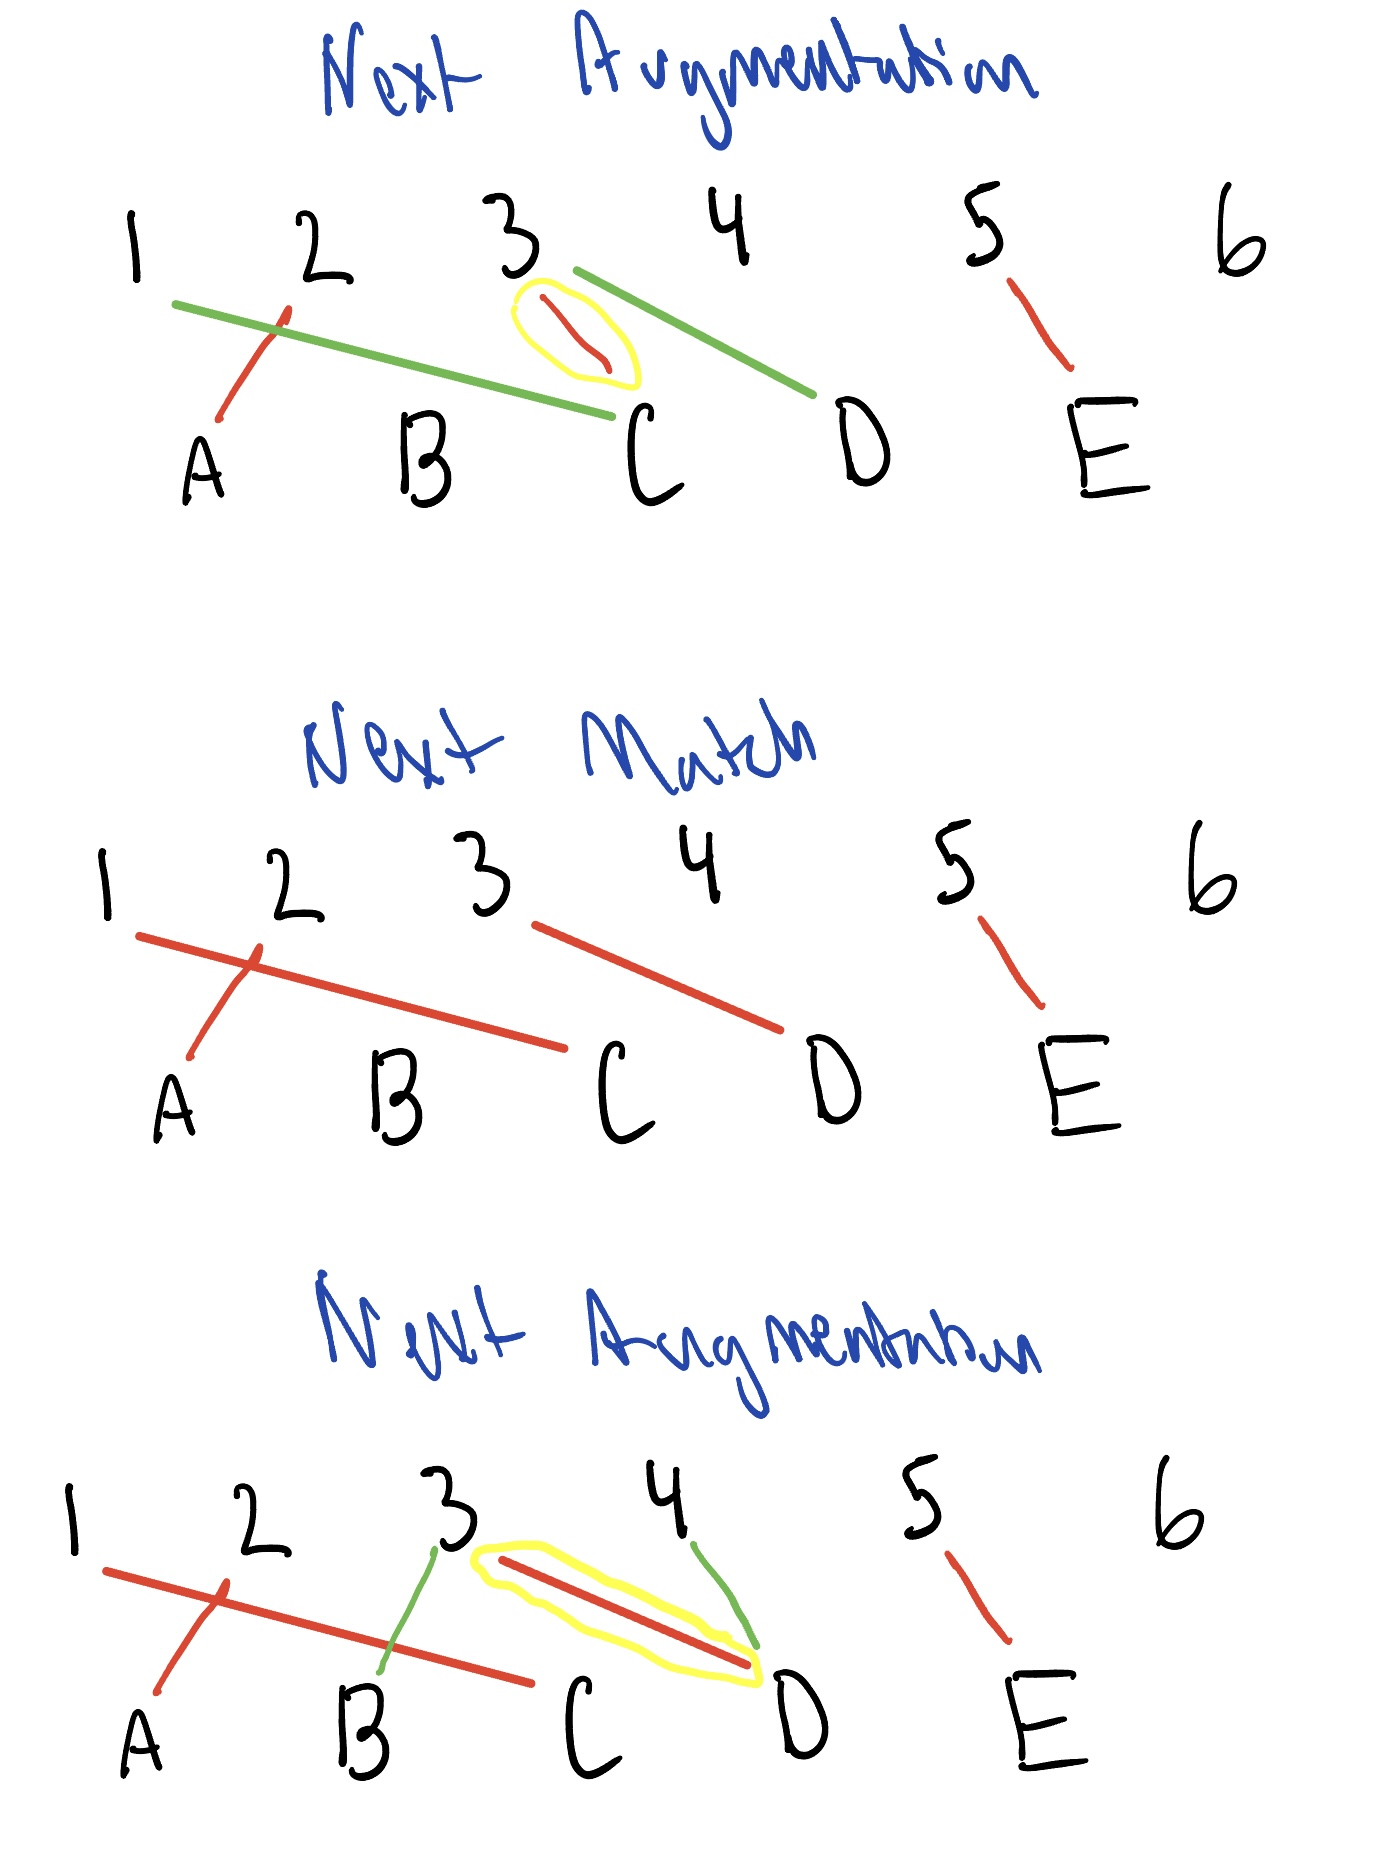
\includegraphics[width=.75\textwidth]{fall2022/psets/ps6/IMG_0011.jpg}\\
    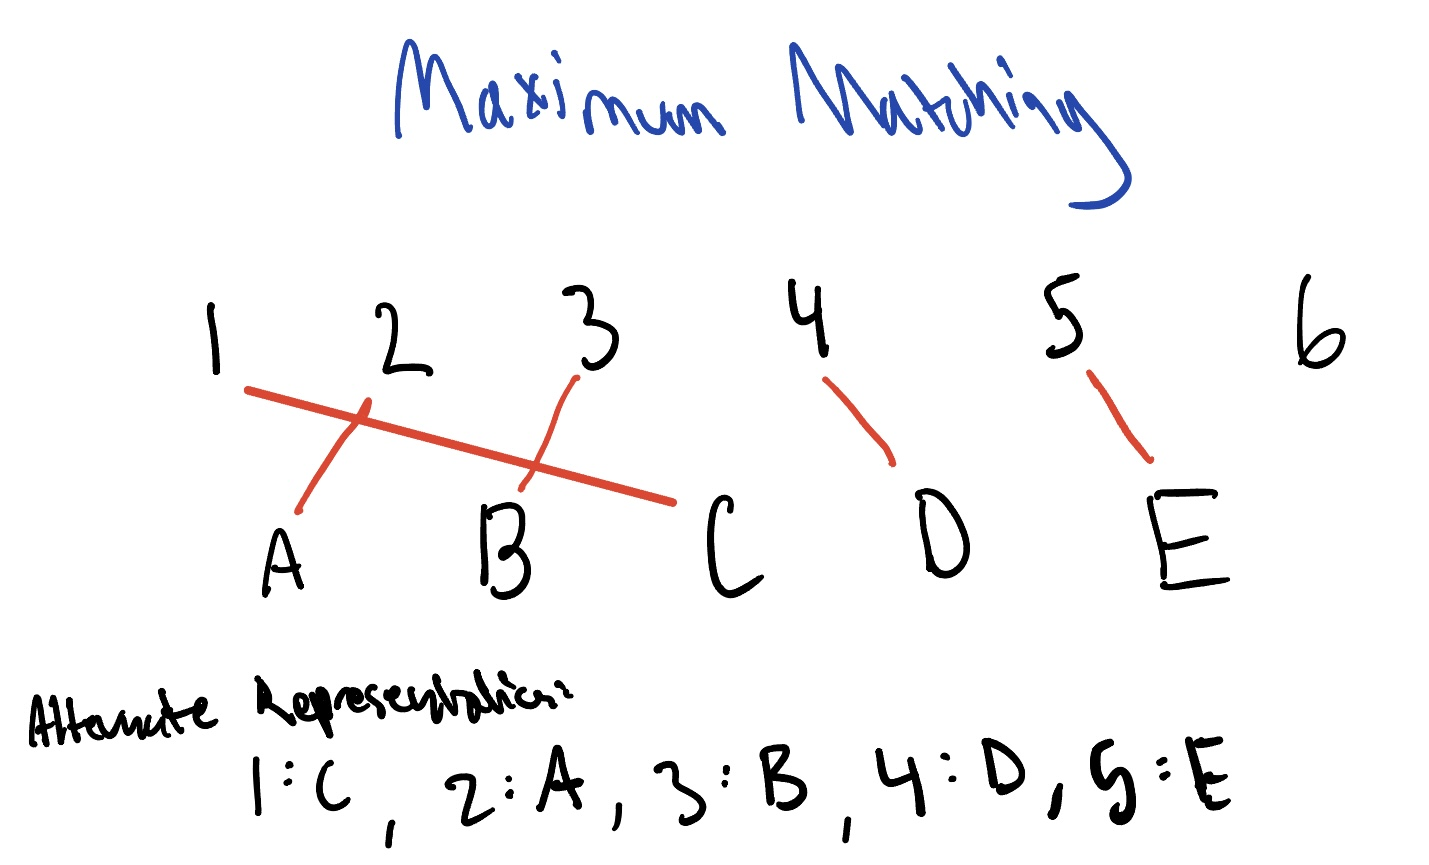
\includegraphics[width=.75\textwidth]{fall2022/psets/ps6/IMG_0012.jpg}\\

    \item The Lyber app also allows users to schedule trips in advance. One Lyber driver receives the following pre-programmed trips scheduled by 4 different users (all of them need multiple rides on the same day):
    \begin{itemize}
        \item User A: one trip from 10 to 10:29, another from 11 to 11:59, another from 12:15 to 12:29, and another from 13 to 13:29.
        \item User B: one trip from 10:15 to 11:14, another from 11:30 to 12:14, and another from 12:45 to 13:14.
        \item User C: one trip from 10:30 to 11:44, another from 12:30 to 12:59, and another from 13:15 to 13:44.
        \item User D: one trip from 10 to 10:44, another from 11:15 to 11:29, another from 12 to 12:44, and another from 13:30 to 13:59.
    \end{itemize}
    The Lyber driver wants to maximize the total number of different rides, because they earn a fixed rate per ride. (The driver is \textit{not} trying to maximize the driving time). 

    We also assume for simplicity that the driver needs no time to move between different rides (i.e., it is possible that one ride finishes at 10:29 and the next one starts immediately at 10:30). 

    Use a greedy algorithm that we saw in class to find a maximum-sized set of non-conflicting rides.  State which algorithm you are using, how you are applying it to this ride-selection problem, and write down the order in which the greedy algorithm selects the rides in the solution. \\
    
    Solution: Within this problem, we will be using the greedy algorithm for interval scheduling shown in class. In particular, we will use this algorithm by treating all the desired ride times as intervals, where we utilize the greedy interval scheduling algorithm to select the maximum number of possible rides. This algorithm states that once we sort the intervals in increasing order by end time, we can find an optimal solution (to maximize interval count) by selecting the earliest ending intervals continuously, ensuring that none conflict until we run out of intervals. This algorithm uses the fact that greedy stays ahead, proved in class in Claim 2.4 Lecture 13. Keeping this in mind, the optimal solution is as follows: \\
    
    Interval solution: 
    $$
    (10 \to 10:29), (11:15 \to 11:29), (11:30 \to 12:14), (12:15 \to 12:29), 
    $$
    
    $$
    (12:30 \to 12:59), (13 \to 13:29), (13:30 \to 13:59)
    $$

    
    \end{enumerate}

 \item (EthiCS Reflection) 
 Suppose there are two patients in need of an immediate kidney transplant, but only one donor is currently available. The donor’s kidney is compatible with both patients. Patient A is 30 years old, and is expected to live 6 additional years as a result of the transplant. Patient B is 60 years old, and is expected to live 10 additional years as a result of the transplant. {\em All else being equal} (e.g., both patients have an urgent need for the transplant; both patients have been on the kidney exchange waiting list for the same length of time), \underline{\textbf{which patient should the kidney go to, and why?}} Your response should take the form of a short paragraph (3-4 sentence) reflection. {\em In explaining your ethical reasoning about the case, be sure to draw on at least one concept discussed in class.} \\
 
 All else being equal, I believe the kidney should go to Patient A. My reasoning can be explained using something similar to the needs-based approach to making decisions, specifically using the Maximin decision principle where we pick a distribution where the person who is least well off is better off than the least well of person in any other distribution. Furthermore, we can use a total-welfare-over-lifetime approach to assessing who to select as the least well off in this situation. To, me, I ethically determined the least well off to be the individual who was projected to live the least even after receiving the transplant. Patient  $A$ was projected to live to $36$ while patient $B$ was projected to live until $70$ with the transplant, so I selected patient $A$ as the individual to donate the kidney to since they would have less time spent to enjoy their life on Earth overall, while person $B$ already lived longer than the projection for patient $A$.

 \item (Vertex-Weighted Matching)
        For a graph $G=(V,E)$ and a subset $F\subseteq E$, 

        let $V(F)$ denote the set $\bigcup_{f \in F}f$ of 
        vertices that are an endpoint of at least one edge in $F$.
        \begin{enumerate}
        \item Prove that if $G=(V,E)$ is a graph and $M\subseteq E$ is a matching in $G$, then there is a maximum-size matching $M'$ such that $V(M)\subseteq V(M')$.  (Hint: consider constructing a maximum matching via augmenting paths, but starting with $M_0=M$ rather than $M_0=\emptyset$. What can you say about the $V(M_i)$'s?) \label{part:monotonicity} \\
        
        Suppose we start with $M_0 = M$ rather than $\emptyset$. If $M$ was already a maximum-size matching, then $M_0 = M'$ and easily $V(M) \subseteq V(M')$. Thus, suppose $M_0$ is not already a maximum matching. Because $M_0$ is not maximum matching, it follows that $\exists$ some augmenting path $P$ by Theorem 4.4 (Berge's Theorem) provided in Lecture 13. We use the maximum matching algorithm provided in Definition 4.1 and Lemma 4.2 to find the next match iteration, $M_1$. Specifically, we use the path $P$ and define it as an alternating walk among some edges ${\{v_0, v_1\},  \{v_0, v_1\}, \dots, \{v_{l-1}, v_{l}\}}$. Just as in that maximum matching algorithm, we keep $v_0$ and $v_{l}$ as unmatched, and have for every $i=1, 2, \dots, l-1$, 
        $$\{v_{i-1}, v_i\} \in M \iff \{v_{i}, v_{i+1}\} \in E - M$$, where $E$ is the entire edge set. Then, by using this augmenting path, we find that the next matching in the iteration $M_1$ is simply 
        $$
        M_{1} = (M - \{\{v_1, v_2\}, \{v_3, v_4\}, \dots , \{v_{l−2}, v_{l-1}\}\}) \cup \{\{v_0, v_1\}, \{v_2, v_3\}, \dots , \{v_{l-1}, v_l\}\}
        $$
        In other words, $M_1$, and without loss of generality every successive $M_j$, consists of the edges that are in $M_0$ but not in the augmented path, along with the edges in the augmented path that are not in $M_0$. Thus, we must consider the edges in $M_0$ that are removed. Suppose there is an edge represented with vertices $\{v_{k}, v_{k+1}\}$in $P$ that would be removed since it was in $M_0$. There may be multiple, but we generalize this by choosing all such arbitrary edges. Note that by definition of the algorithm, there must be another preceding edge such that contains $v_k$ and an edge that contains $v_{k+1}$. In particular, there must be an originally unmatched vertex $v_{k-1}$ and unmatched vertex $v_{k+2}$ in the augmented path such that new edges $\{v_{k-1}, v_k\}$ and $\{v_{k+1}, v_{k+2}\}$ are contained within the augmented path. These edges satistfy the condition of not being contained within $M_0$ but being contained within the augmented path $P$. Thus, they as defined by our algorithm, they are contained within $M_1$. Note then that the vertices $v_k$ and $v_{k+1}$ which originally had an edge that was removed are indeed still contained within the successive matching $M_1$. Thus, edges in $M_0$ are either not contained within the augmented path in which case they automatically are included in $M_1$, or they are in the augmented path, in which the formation of new edges allows those vertices to remain in $M_1$. Thus, we have proved that for any $v in V(M_0)$, it follows that $v \in V(M_1)$. Thus, $V(M_0) \subseteq V(M_1)$. \\
        
        Note that above was similar to a base case for an inductive proof, since we proved the case true for the initial state of $M_0 = M$. However, even $M_1$ may not be a maximum matching, so we must keep repeating the process outlined above, such that at the $i_{th}$ iteration, we treat $M_{i-1}$ as the initial state given that $M_{i-1} \neq M^*$, a maximum matching. 
        Similar to the proof given above then, assume the first $k$ iterations of augmentation hold, such that $V(M_0) \subseteq V(M_{k})$. We wish to prove that $V(M_0) \subseteq V(M_{k+1})$. Treat $M_k$ as the initial state, and follow the steps outlined in the proof of the base case. It then follows that $V(M_k) \subseteq V(M_{k+1}$. Then, however, because $V(M_0) \subseteq V(M_{k})$, it follows that $V(M_0) \subseteq V(M_{k+1})$. Thus, we have completed the proof via induction on the number of augmentations we have performed, and we can keep repeating the process until we find a maximum possible matching, knowing that all vertices of the original matching will be contained in the vertex set of the maximum matching. 
        \item   In the Embedded EthiCS module, we saw how simply maximizing the {\em size} of a matching may not always be the right objective.  Thus, it is natural to consider weighted versions of the matching problem. Suppose we
        we consider vertex-weighted graphs $G = (V,E,w)$, $w$ is an array specifying a nonnegative edge weight $w(v)$ for every $v\in V$.  (For example, the weight assigned to a patient might correspond to the number of extra years of life they would gain from a donation.)
          The goal of the {\em vertex-weighted maximum matching problem} is to find a matching $M$ maximizing its {\em total weight} $$w(M) = \sum_{\{u,v\}\in M} (w(u)+w(v)).$$
        (This corresponds to the utilitarian objective discussed in Embedded EthiCS module.)
        Using Part~\ref{part:monotonicity}, prove that every graph $G$ has a matching $M^*$ that simultaneously maximizes both total weight and size.  That is, for every matching $M$ in $G$, we have
        both $w(M)\leq w(M^*)$ and $|M|\leq |M^*|$. \\
        
        Consider any arbitrary non maximum matching $M$ that has a vertex set $V(M)$. Based on the result of part $3a$, it follows that we can turn any such $M$ into a maximum matching $M'$ such that $V(M) \subseteq V(M')$. Suppose $v_1, v_2, \cdots v_m$ are the vertices of $V(M)$. Then we can let $v_1, v_2, \cdots v_m, u_1, u_2, \cdots u_n$ be the vertices of $V(M')$, where $\{u_1, u_2, \cdots u_n\} = V(M') - V(M)$. Let $w(M) = \sum_1^m v_i$. Then, because all vertex weights are nonnegative, it follows that 
        $$w(M') = \sum_{i=1}^m v_i + \sum_{j=1}^n u_j = w(M) + \sum_{j=1}^n u_j \geq w(M).$$. Thus, this proves that maximum matches have total weighting at least as large as any match that contains vertices that are a subset of that particular maximum match. \\
        
        Now, consider that because $G$ has a finite number of vertices and edges, it must have a finite number of maximum matches. Intuition for this can be gained from the pigeonhole principle. Now, let's denote these finite number of maximum matches as $w_1, w_2, \cdots w_y$. Now, choose the particular $w_z$ where $z \in \{1, 2, \cdots y\}$ such that $w_z \geq w_1, w_z \geq w_2, \cdots, w_z \geq w_y$. That is, choose the maximum matching out of the finite set that has the maximum weighting compared to all other maximum matches. This is the matching that is equivalent to the matching we are looking for, $M^*$. This can be proved by the fact that we just showed this matching is larger in weight than all other maximum matches, and is larger in weighting than all subsets of $V(M^*)$ as proved above. Again, since any smaller match $M$ can be mapped to a maximum matching via the augmentation strategy, their vertex set would already be a subset of one of the maximum matches' vertex sets. Thus, we have found the optimal $M^*$ and proved its existence. 

        \item (optional\footnote{This problem won't make a difference between N, L, R-, and R grades. As this problem is purely extra credit, course staff will deprioritize questions about this problem at office hours and on Ed.}) Explain why the same holds for the maximin objective discussed in the Embedded EthiCS module.  That is, there is always a matching $M$ that simultaneously maximizes the maximin objective and $|M|$. 
        \end{enumerate}
        

\item (Edge-Weighted Bipartite Matching) 
  Instead of considering vertex weights, we could instead study matching on
{\em edge-weighted} bipartite graphs $G = (V,E,w)$, where $w$ is an array specifying a nonnegative edge weight $w(e)$ for every $e\in E$.  

   The goal of the {\em edge-weighted maximum matching problem} is to find a matching $M$ maximizing $$w(M) = \sum_{e\in M} w(e).$$
   \begin{enumerate}
    \item Construct an edge-weighted bipartite graph $G = (V,E,w)$ such that there is no matching $M$ in $G$ that simultaneously maximizes the weight $w(M)$ and the size $|M|$.  Thus, there can be an inherent tension between these two objectives. \\
    
    Suppose we define the two distinct vertex sets of the bipartite graph such that no pair of vertices within an individual set contain an edge connecting them as $u_1, u_2, \cdots, u_n$ and $v_1, v_2, \cdots v_m$ where the size of the first vertex set of $G$ is $n$ and the size of the second vertex set of $G$ is $m$. We have $V = u_1, u_2, \cdots, u_n, v_1, v_2, \cdots v_m$. Then, whichever is smaller, $n$ or $m$, pick that number of vertices from the other vertex set. That is, if $n$ is smaller, pick $n$ vertices from $v_1, v_2, \cdots v_m$ or vice versa. We only need the smaller number because this smaller number is the limit of edges possible in the maximum matching by definition. Without loss of generality, suppose it is $n \leq m$, such that we choose $v_1, v_2, \cdots v_n$. Now consider this remaining vertex set in conjunction with the original smaller vertex set $u_1, u_2, \cdots u_n$. We will create $n$ edges at first by creating edges $\{u_1, v_1\}, \{u_2, v_2\}, \cdots, \{u_n, v_n\}$. Now choose some arbitrary two edges, $\{u_i, v_i\}, \{u_j, v_j\}$. Create another edge between $u_i$ and $v_j$, that is, an edge $\{u_i, v_j\}$. We will now consider assigning weights. Assign weight such that $w(\{u_i, v_j\}) > w(\{u_i, v_i\}) + w(\{u_j, v_j\})$, and further assign weight such that for all $k = 1, 2, \dots, n : k \neq i, j$ we have $w(k) = c$. That is, we want the weight on all other possible edges that are not the edges $\{u_i, v_i\}, \{u_j, v_j\}, or \{u_i, v_j\}$ to be the same. Let all edges discussed define $E$, all vertices discussed define $V$, and all weights discussed define $w$. Then, note that we have constructed a desired bipartite graph $G = (V, E, w)$ such that there is no matching $M$ in $G$ that simultaneously maximizes $w(M)$ and $|M|$. In this graph, the maximum size matching set would be of size $n$ and contain edges $\{u_1, v_1\}, \{u_2, v_2\}, \cdots, \{u_n, v_n\}$, whereas the maximum weight matching would contain $\{u_i, v_j\}$ and all other edges $\{u_1, v_1\}, \{u_2, v_2\}, \cdots, \{u_n, v_n\}$ EXCEPT FOR $\{u_i, v_i\}$ and $\{u_j, v_j\}$, which therefore only has cardinality $n-1$. Thus, we have constructed the desired graph, and our work is complete. 

    \item (optional\footnotemark[1])
  
    One real-life constraint in kidney exchange is that donors $d$ are often associated with a particular patient $p$ (e.g. a close family member) such that $d$ is only willing to donate a kidney if $p$ receives a kidney from someone.  ($d$ would donate their kidney directly to $p$ if they could, but they are incompatible.) 
    Suppose we have an (unweighted) bipartite graph $G=(V_0\cup V_1,E)$ representing $n$ such donor-patient pairs, i.e. $V_0=\{d_0,d_1,\ldots,d_{n-1}\}$, $V_1 = \{p_0,p_1,\ldots,p_{n-1}\}$, where $p_i$ is the patient associated with donor $d_i$. We assume $\{d_i,p_i\}\notin E$ for each $i$.   Our goal is to find a matching $M$ of the largest possible size $|M|$, subject to the constraint that $d_i$ is matched in $M$ only if $p_i$ is matched in $M$. 

    Show that we can reduce this constrained version of the maximum matching problem to finding a maximum-weight {\em perfect} matching in an appropriate edge-weighted bipartite graph, where
    a perfect matching is a matching that matches all the vertices in the graph. (Hint: add edges $\{d_i,p_i\}$ with appropriate edge weights.) 
    \end{enumerate}

\end{enumerate}
\end{document}
